\documentclass[twocolumn]{article}
\usepackage{amsmath,amssymb,amsthm,kotex,paralist}

\usepackage[skipabove=10pt,align=center]{mdframed}

\newcommand\ov[2]{\ensuremath{\overline{#1#2}}}

\setlength{\parindent}{0pt}
%%%%
\begin{document}

\centering
\begin{mdframed}
\(\square ABCD\)의 외접원이 존재한다.
\end{mdframed}

\(\Updownarrow\)

\begin{mdframed}
네 점이 한 원 위에 있다.
\end{mdframed}

\(\Updownarrow\)

\begin{mdframed}
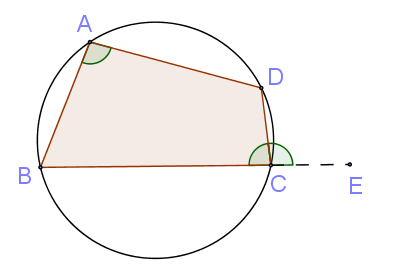
\includegraphics{1}\\
\(\angle A+\angle C=180^\circ\)\\
\(\angle A=\angle DCT\)
\end{mdframed}

\(\Updownarrow\)

\begin{mdframed}

\includegraphics{2}\\
\(\angle BAC=\angle BDC\)
\end{mdframed}

\(\Updownarrow\)

\begin{mdframed}
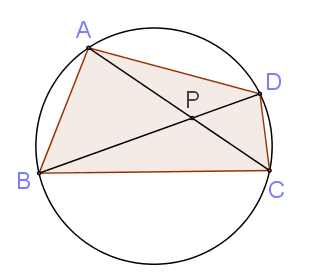
\includegraphics{3}\\
\(\ov PA\times\ov PC=\ov PB+\ov PD\)
\end{mdframed}

\(\Updownarrow\)

\begin{mdframed}

\includegraphics{4}\\
\(\ov QA\times\ov QD=\ov QB+\ov QC\)
\end{mdframed}

\newpage
\begin{mdframed}
\(\square ABCD\)의 내접원이 존재한다.
\end{mdframed}

\(\Updownarrow\)

\begin{mdframed}
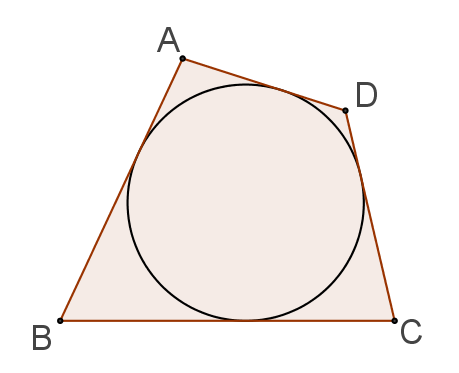
\includegraphics{5}\\
\(\ov AB+\ov CD=\ov AD+\ov BC\)
\end{mdframed}

\vspace{0.13\textheight}

\begin{mdframed}
직선 \(l\)이 원 \(O\)에 접한다.
\end{mdframed}

%\(\Updownarrow\)
%
%\begin{mdframed}
%직선 \(l\)과 원 \(O\)의 교점이 1개이다.
%\end{mdframed}

\(\Updownarrow\)

\begin{mdframed}
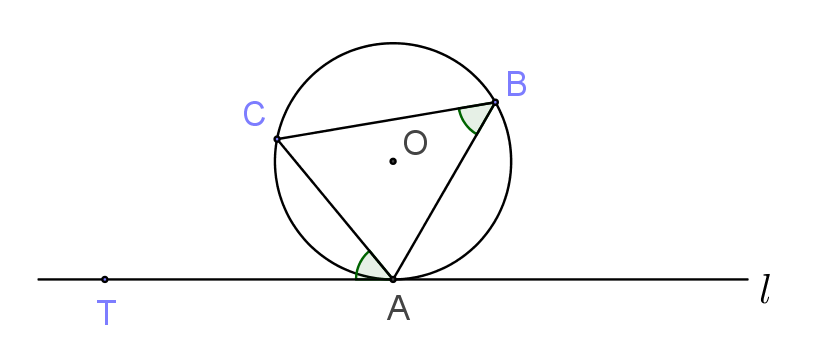
\includegraphics{6}\\
\(\angle ABC=\angle CAT\)
\end{mdframed}

\(\Updownarrow\)

\begin{mdframed}
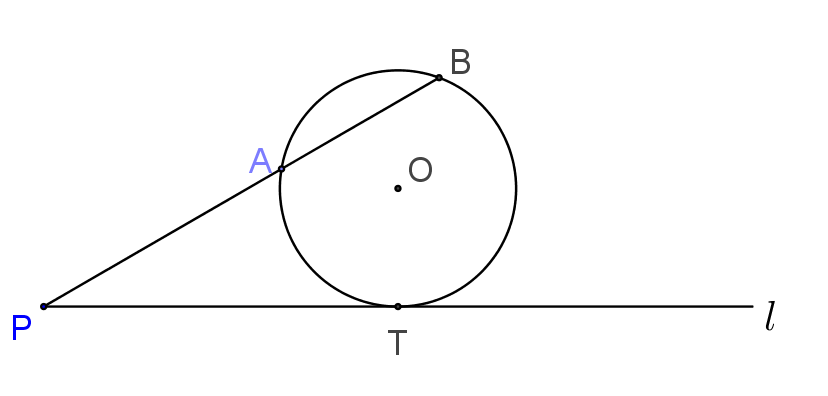
\includegraphics{7}\\
\(\ov PA\times\ov PB=\ov PT^2\)
\end{mdframed}

\end{document}